\documentclass[12pt,a4paper,openany]{article}
%%%% JNLP 
\usepackage{lmodern}
\usepackage{xcolor}
\usepackage[utf8]{inputenc}
\usepackage[T1]{fontenc}
\usepackage[francais]{babel}
\usepackage[top=1.7cm, bottom=1.7cm, left=1.7cm, right=1.7cm]{geometry}
\usepackage{pdfpages}
%\usepackage[frenchb]{babel}
%\usepackage{layout}
%\usepackage{setspace}
%\usepackage{soul}
%\usepackage{ulem}
%\usepackage{eurosym}
%\usepackage{bookman}
%\usepackage{charter}
%\usepackage{newcent}
%\usepackage{lmodern}
%\usepackage{mathpazo}
%\usepackage{mathptmx}
%\usepackage{url}
%\usepackage{verbatim}
%\usepackage{moreverb}
%\usepackage{wrapfig}
%\usepackage{amsmath}
%\usepackage{mathrsfs}
%\usepackage{asmthm}
%\usepackage{makeidx}
\usepackage{tikz} %Vectoriel
\usepackage{listingsutf8}
\usepackage{fancyhdr}
\usepackage{multido}
\usepackage{amssymb}

%\include{/home/satenske/cours/listing_algo} %prise en charge du langage algo

\date{\today}

\chead{Ce document est un outil pédagogique il ne vaut en aucun cas contrat}
\rhead{}
\lhead{}

\lfoot{Université Paul Sabatier Toulouse III}
\rfoot{--~\thepage~--}
\cfoot{}
\makeatletter
\def\clap#1{\hbox to 0pt{\hss #1\hss}}%
\def\ligne#1{%
\hbox to \hsize{%
\vbox{\centering #1}}}%
\def\haut#1#2#3{%
\hbox to \hsize{%
\rlap{\vtop{\raggedright #1}}%
\hss
\clap{\vtop{\centering #2}}%
\hss
\llap{\vtop{\raggedleft #3}}}}%
\def\bas#1#2#3{%
\hbox to \hsize{%
\rlap{\vbox{\raggedright #1}}%
\hss \clap{\vbox{\centering #2}}%
\hss
\llap{\vbox{\raggedleft #3}}}}%
\def\maketitle{%
\thispagestyle{empty}\vbox to \vsize{%
\haut{}{\@blurb}{}
\begin{flushleft}
	\vspace{1cm}
	Antoine de \bsc{Roquemaurel}\\ 
	Mathieu \bsc{Soum}\\
	Geoffroy \bsc{Subias}\\
	Marie-Ly \bsc{Tang}\\
	\textit{Groupe B}\\
\end{flushleft}
\begin{flushright}
	\vspace{-3cm}
	Pour Monsieur \bsc{Millan} (Client)\\
	Pour Madame \bsc{Kross} (Tuteur) \\
	Pour Monsieur \bsc{Marquié} (Correcteur)

\end{flushright}
\vfill
\vspace{1cm}
\begin{flushleft}
\usefont{OT1}{ptm}{m}{n}
\huge \@title
\end{flushleft}
\par
\hrule height 4pt
\par
\begin{flushright}
\usefont{OT1}{phv}{m}{n}
\Large \@author
\par
\end{flushright}
\vspace{1cm}
\vfill
\vfill
\bas{}{\@location, le \@date}{}
}%
\cleardoublepage
}
\def\date#1{\def\@date{#1}}
\def\author#1{\def\@author{#1}}
\def\title#1{\def\@title{#1}}
\def\location#1{\def\@location{#1}}
\def\blurb#1{\def\@blurb{#1}}
\date{\today}
\author{}
\title{}
\location{Amiens}\blurb{}
\makeatother
\title{Cahier des Charges Fonctionnel}
\author{Bibliothèque d'objets graphiques UML}

\location{Toulouse}
\blurb{%
Université Paul Sabatier -- Toulouse III\\
IUT A - Toulouse Rangueil\\
\textbf{Projet tutoré}\\[1em]
}%
\pagestyle{fancy}
\begin{document}
	\maketitle
	\newpage
	\tableofcontents
	\newpage
	\section{Contexte}
	\subsection{Présentation du groupe projet}
	Notre groupe projet est composé de quatre étudiants de deuxième année de DUT\footnote{Diplôme Universitaire de Technologie} Informatique à l'IUT\footnote{Institut Universitaire de Technologie} A de Toulouse, voici la composition de l'équipe: 
	\begin{itemize}
		\item Antoine de \bsc{Roquemaurel} 
		\item Mathieu \bsc{Soum} 
		\item Geoffroy \bsc{Subias}
		\item Marie-Ly \bsc{Tang} 
	\end{itemize}
	Nous avons monté ce groupe, car nos compétences sont complémentaires et que nous savons déjà comment chacun travaille. Antoine de \bsc{Roquemaurel} et Mathieu \bsc{Soum} sont spécialisés en programmation par objet, Geoffroy \bsc{Subias} maîtrise la modélisation UML\footnote{Unified Modelling Language} et Marie-Ly \bsc{Tang} 
	s'occupera principalement de l'organisation et de la gestion de projet.
		
	\subsection{Présentation du commanditaire}
	Monsieur Thierry \bsc{Millan} est un enseignant à l'IUT A Toulouse et chercheur à l'IRIT\footnote{Institut de Recherche Informatique de Toulouse}
	\subsection{Présentation du projet}
		L'objectif du projet est de réaliser une bibliothèque d'objets graphiques représentant les 
		différents éléments de modélisation de la norme UML 2.
		\subsubsection*{Risques}
		\begin{center}
		\begin{tabular}{|p{5.5cm}|c|p{6.5cm}|c|}
				\hline
				\textbf{Risques} & \textbf{Pertinence} & \textbf{Solution} & \textbf{Responsable} \\
				\hline
				Crash du disque dur contenant le projet & Moyenne & Avoir le projet sur plusieurs périphériques & Mathieu\\
				\hline
				Non respect du besoin du client & Moyenne & Voir le client régulierement (environ toutes les deux semaines) & Marie-Ly\\ 
				\hline
				Retard du projet & Haute & Respecter scrupuleusement le planning et le Gantt & Geoffroy\\
				\hline
				Évolution du besoin du client & Moyenne &  Nous travaillerons par incréments, 
				en rencontrant régulièrement le client  nous aurons le temps d'implémenter ses besoins et 
				ce qui évitera les demandes de dernières minutes & Marie-Ly \\ 
				\hline
				Mauvaise coordination entrainant des divergences de développement& Faible & Utiliser une plateforme de travail collaboratif (Redmine) afin que
				chaque membre soit au courant des évolutions du projet & Antoine \\
				\hline
				Indisponibilité du serveur permettant le travail collaboratif & Haute& Héberger le serveur à domicile pour effectuer une maintenance rapide.
				Ajout d'un onduleur & Antoine  \\
				\hline
			\end{tabular}
		\end{center}	
	\section{Description de la demande}
	\paragraph{}
		Le cahier des charges fonctionnel sera évolutif car le projet sera incrémental et chaque incrément devra 
		être validé par le client. Le cycle de développement sera un cycle à incrément court (Deux à trois semaines).
	\paragraph{}
		Le logiciel sera codé en Java et devra être utilisable comme composant par un autre logiciel.\\
	\paragraph{Objectif du client à court terme} Au terme de notre premier incrément, l'objectif sera
	de pouvoir utiliser des fonctionnalités de base telles que le dessin de diagramme simple, sans aucune
	contrainte vis-à-vis de la norme UML 2.0.
	\paragraph{Objectif du client à long terme}
	Le projet une fois terminé devra permettre à l'utilisateur de dessiner des diagrammes UML de séquence ou de classe.\\
	Selon l'évolution du projet, le client se réserve le droit de modifier ces conditions pour y
	intégrer des contraintes vis-à-vis de la norme UML 2.0 et de différencier les types de diagramme lors de leur conception. 
	
	\subsection{Évaluation des fonctions}
%	% Graphic for TeX using PGF
% Title: /home/satenske/cours/projet_IUT/cahierDesCharges/pieuvre.dia
% Creator: Dia v0.97.1
% CreationDate: Thu Oct 13 15:38:07 2011
% For: satenske
% \usepackage{tikz}
% The following commands are not supported in PSTricks at present
% We define them conditionally, so when they are implemented,
% this pgf file will use them.
\ifx\du\undefined
  \newlength{\du}
\fi
\setlength{\du}{15\unitlength}
\begin{tikzpicture}
\pgftransformxscale{1.000000}
\pgftransformyscale{-1.000000}
\definecolor{dialinecolor}{rgb}{0.000000, 0.000000, 0.000000}
\pgfsetstrokecolor{dialinecolor}
\definecolor{dialinecolor}{rgb}{1.000000, 1.000000, 1.000000}
\pgfsetfillcolor{dialinecolor}
\definecolor{dialinecolor}{rgb}{1.000000, 1.000000, 1.000000}
\pgfsetfillcolor{dialinecolor}
\pgfpathellipse{\pgfpoint{17.025000\du}{13.975000\du}}{\pgfpoint{2.975000\du}{0\du}}{\pgfpoint{0\du}{1.675000\du}}
\pgfusepath{fill}
\pgfsetlinewidth{0.020000\du}
\pgfsetdash{}{0pt}
\pgfsetdash{}{0pt}
\definecolor{dialinecolor}{rgb}{0.000000, 0.000000, 0.000000}
\pgfsetstrokecolor{dialinecolor}
\pgfpathellipse{\pgfpoint{17.025000\du}{13.975000\du}}{\pgfpoint{2.975000\du}{0\du}}{\pgfpoint{0\du}{1.675000\du}}
\pgfusepath{stroke}
% setfont left to latex
\definecolor{dialinecolor}{rgb}{0.000000, 0.000000, 0.000000}
\pgfsetstrokecolor{dialinecolor}
\node[anchor=west] at (14.850000\du,14.150000\du){Logiciel UML};
\definecolor{dialinecolor}{rgb}{1.000000, 1.000000, 1.000000}
\pgfsetfillcolor{dialinecolor}
\pgfpathellipse{\pgfpoint{20.265000\du}{7.405000\du}}{\pgfpoint{2.975000\du}{0\du}}{\pgfpoint{0\du}{1.675000\du}}
\pgfusepath{fill}
\pgfsetlinewidth{0.020000\du}
\pgfsetdash{}{0pt}
\pgfsetdash{}{0pt}
\definecolor{dialinecolor}{rgb}{0.000000, 0.000000, 0.000000}
\pgfsetstrokecolor{dialinecolor}
\pgfpathellipse{\pgfpoint{20.265000\du}{7.405000\du}}{\pgfpoint{2.975000\du}{0\du}}{\pgfpoint{0\du}{1.675000\du}}
\pgfusepath{stroke}
% setfont left to latex
\definecolor{dialinecolor}{rgb}{0.000000, 0.000000, 0.000000}
\pgfsetstrokecolor{dialinecolor}
\node[anchor=west] at (18.450000\du,7.300000\du){Utilisateur};
\definecolor{dialinecolor}{rgb}{1.000000, 1.000000, 1.000000}
\pgfsetfillcolor{dialinecolor}
\pgfpathellipse{\pgfpoint{6.765000\du}{19.205000\du}}{\pgfpoint{2.975000\du}{0\du}}{\pgfpoint{0\du}{1.675000\du}}
\pgfusepath{fill}
\pgfsetlinewidth{0.020000\du}
\pgfsetdash{}{0pt}
\pgfsetdash{}{0pt}
\definecolor{dialinecolor}{rgb}{0.000000, 0.000000, 0.000000}
\pgfsetstrokecolor{dialinecolor}
\pgfpathellipse{\pgfpoint{6.765000\du}{19.205000\du}}{\pgfpoint{2.975000\du}{0\du}}{\pgfpoint{0\du}{1.675000\du}}
\pgfusepath{stroke}
\definecolor{dialinecolor}{rgb}{1.000000, 1.000000, 1.000000}
\pgfsetfillcolor{dialinecolor}
\pgfpathellipse{\pgfpoint{7.515000\du}{13.455000\du}}{\pgfpoint{2.975000\du}{0\du}}{\pgfpoint{0\du}{1.675000\du}}
\pgfusepath{fill}
\pgfsetlinewidth{0.020000\du}
\pgfsetdash{}{0pt}
\pgfsetdash{}{0pt}
\definecolor{dialinecolor}{rgb}{0.000000, 0.000000, 0.000000}
\pgfsetstrokecolor{dialinecolor}
\pgfpathellipse{\pgfpoint{7.515000\du}{13.455000\du}}{\pgfpoint{2.975000\du}{0\du}}{\pgfpoint{0\du}{1.675000\du}}
\pgfusepath{stroke}
% setfont left to latex
\definecolor{dialinecolor}{rgb}{0.000000, 0.000000, 0.000000}
\pgfsetstrokecolor{dialinecolor}
\node at (6.700000\du,18.950000\du){Système };
% setfont left to latex
\definecolor{dialinecolor}{rgb}{0.000000, 0.000000, 0.000000}
\pgfsetstrokecolor{dialinecolor}
\node at (6.700000\du,19.750000\du){d'exploitation};
% setfont left to latex
\definecolor{dialinecolor}{rgb}{0.000000, 0.000000, 0.000000}
\pgfsetstrokecolor{dialinecolor}
\node at (7.515000\du,13.455000\du){Mémoire};
\definecolor{dialinecolor}{rgb}{1.000000, 1.000000, 1.000000}
\pgfsetfillcolor{dialinecolor}
\pgfpathellipse{\pgfpoint{11.865000\du}{7.205000\du}}{\pgfpoint{2.975000\du}{0\du}}{\pgfpoint{0\du}{1.675000\du}}
\pgfusepath{fill}
\pgfsetlinewidth{0.020000\du}
\pgfsetdash{}{0pt}
\pgfsetdash{}{0pt}
\definecolor{dialinecolor}{rgb}{0.000000, 0.000000, 0.000000}
\pgfsetstrokecolor{dialinecolor}
\pgfpathellipse{\pgfpoint{11.865000\du}{7.205000\du}}{\pgfpoint{2.975000\du}{0\du}}{\pgfpoint{0\du}{1.675000\du}}
\pgfusepath{stroke}
% setfont left to latex
\definecolor{dialinecolor}{rgb}{0.000000, 0.000000, 0.000000}
\pgfsetstrokecolor{dialinecolor}
\node at (11.865000\du,7.205000\du){Diagramme};
% setfont left to latex
\definecolor{dialinecolor}{rgb}{0.000000, 0.000000, 0.000000}
\pgfsetstrokecolor{dialinecolor}
\node at (11.865000\du,8.005000\du){de classe};
\definecolor{dialinecolor}{rgb}{1.000000, 1.000000, 1.000000}
\pgfsetfillcolor{dialinecolor}
\pgfpathellipse{\pgfpoint{26.115000\du}{18.455000\du}}{\pgfpoint{2.975000\du}{0\du}}{\pgfpoint{0\du}{1.675000\du}}
\pgfusepath{fill}
\pgfsetlinewidth{0.020000\du}
\pgfsetdash{}{0pt}
\pgfsetdash{}{0pt}
\definecolor{dialinecolor}{rgb}{0.000000, 0.000000, 0.000000}
\pgfsetstrokecolor{dialinecolor}
\pgfpathellipse{\pgfpoint{26.115000\du}{18.455000\du}}{\pgfpoint{2.975000\du}{0\du}}{\pgfpoint{0\du}{1.675000\du}}
\pgfusepath{stroke}
% setfont left to latex
\definecolor{dialinecolor}{rgb}{0.000000, 0.000000, 0.000000}
\pgfsetstrokecolor{dialinecolor}
\node[anchor=west] at (23.865000\du,18.055000\du){Érgonomie};
\pgfsetlinewidth{0.020000\du}
\pgfsetdash{}{0pt}
\pgfsetdash{}{0pt}
\pgfsetbuttcap
{
\definecolor{dialinecolor}{rgb}{0.000000, 0.000000, 0.000000}
\pgfsetfillcolor{dialinecolor}
% was here!!!
\definecolor{dialinecolor}{rgb}{0.000000, 0.000000, 0.000000}
\pgfsetstrokecolor{dialinecolor}
\pgfpathmoveto{\pgfpoint{11.602261\du}{8.881932\du}}
\pgfpatharc{178}{5}{4.432200\du and 4.432200\du}
\pgfusepath{stroke}
}
\pgfsetlinewidth{0.020000\du}
\pgfsetdash{}{0pt}
\pgfsetdash{}{0pt}
\pgfsetmiterjoin
\pgfsetbuttcap
{
\definecolor{dialinecolor}{rgb}{0.000000, 0.000000, 0.000000}
\pgfsetfillcolor{dialinecolor}
% was here!!!
\definecolor{dialinecolor}{rgb}{0.000000, 0.000000, 0.000000}
\pgfsetstrokecolor{dialinecolor}
\pgfpathmoveto{\pgfpoint{10.495965\du}{13.455000\du}}
\pgfpathcurveto{\pgfpoint{13.653265\du}{13.455000\du}}{\pgfpoint{10.886735\du}{13.975000\du}}{\pgfpoint{14.044035\du}{13.975000\du}}
\pgfusepath{stroke}
}
\pgfsetlinewidth{0.020000\du}
\pgfsetdash{}{0pt}
\pgfsetdash{}{0pt}
\pgfsetmiterjoin
\pgfsetbuttcap
{
\definecolor{dialinecolor}{rgb}{0.000000, 0.000000, 0.000000}
\pgfsetfillcolor{dialinecolor}
% was here!!!
\definecolor{dialinecolor}{rgb}{0.000000, 0.000000, 0.000000}
\pgfsetstrokecolor{dialinecolor}
\pgfpathmoveto{\pgfpoint{9.748052\du}{19.205000\du}}
\pgfpathcurveto{\pgfpoint{12.905352\du}{19.205000\du}}{\pgfpoint{12.279629\du}{16.023002\du}}{\pgfpoint{14.654629\du}{14.998002\du}}
\pgfusepath{stroke}
}
\pgfsetlinewidth{0.020000\du}
\pgfsetdash{}{0pt}
\pgfsetdash{}{0pt}
\pgfsetmiterjoin
\pgfsetbuttcap
{
\definecolor{dialinecolor}{rgb}{0.000000, 0.000000, 0.000000}
\pgfsetfillcolor{dialinecolor}
% was here!!!
\definecolor{dialinecolor}{rgb}{0.000000, 0.000000, 0.000000}
\pgfsetstrokecolor{dialinecolor}
\pgfpathmoveto{\pgfpoint{25.427412\du}{16.815366\du}}
\pgfpathcurveto{\pgfpoint{25.362412\du}{16.660366\du}}{\pgfpoint{20.905641\du}{18.211083\du}}{\pgfpoint{18.395641\du}{15.471183\du}}
\pgfusepath{stroke}
}
% setfont left to latex
\definecolor{dialinecolor}{rgb}{0.000000, 0.000000, 0.000000}
\pgfsetstrokecolor{dialinecolor}
\node[anchor=west] at (14.150000\du,11.650000\du){FP1};
% setfont left to latex
\definecolor{dialinecolor}{rgb}{0.000000, 0.000000, 0.000000}
\pgfsetstrokecolor{dialinecolor}
\node[anchor=west] at (10.980000\du,12.915000\du){FC1};
% setfont left to latex
\definecolor{dialinecolor}{rgb}{0.000000, 0.000000, 0.000000}
\pgfsetstrokecolor{dialinecolor}
\node[anchor=west] at (10.350000\du,17.600000\du){FC2};
% setfont left to latex
\definecolor{dialinecolor}{rgb}{0.000000, 0.000000, 0.000000}
\pgfsetstrokecolor{dialinecolor}
\node[anchor=west] at (19.380000\du,17.965000\du){FC3};
\definecolor{dialinecolor}{rgb}{1.000000, 1.000000, 1.000000}
\pgfsetfillcolor{dialinecolor}
\pgfpathellipse{\pgfpoint{26.520000\du}{10.955000\du}}{\pgfpoint{2.975000\du}{0\du}}{\pgfpoint{0\du}{1.675000\du}}
\pgfusepath{fill}
\pgfsetlinewidth{0.020000\du}
\pgfsetdash{}{0pt}
\pgfsetdash{}{0pt}
\definecolor{dialinecolor}{rgb}{0.000000, 0.000000, 0.000000}
\pgfsetstrokecolor{dialinecolor}
\pgfpathellipse{\pgfpoint{26.520000\du}{10.955000\du}}{\pgfpoint{2.975000\du}{0\du}}{\pgfpoint{0\du}{1.675000\du}}
\pgfusepath{stroke}
% setfont left to latex
\definecolor{dialinecolor}{rgb}{0.000000, 0.000000, 0.000000}
\pgfsetstrokecolor{dialinecolor}
\node at (26.520000\du,10.955000\du){Diagramme};
% setfont left to latex
\definecolor{dialinecolor}{rgb}{0.000000, 0.000000, 0.000000}
\pgfsetstrokecolor{dialinecolor}
\node at (26.520000\du,11.755000\du){de séquence};
\pgfsetlinewidth{0.020000\du}
\pgfsetdash{}{0pt}
\pgfsetdash{}{0pt}
\pgfsetbuttcap
{
\definecolor{dialinecolor}{rgb}{0.000000, 0.000000, 0.000000}
\pgfsetfillcolor{dialinecolor}
% was here!!!
\definecolor{dialinecolor}{rgb}{0.000000, 0.000000, 0.000000}
\pgfsetstrokecolor{dialinecolor}
\pgfpathmoveto{\pgfpoint{18.772026\du}{8.862062\du}}
\pgfpatharc{212}{23}{4.177083\du and 4.177083\du}
\pgfusepath{stroke}
}
% setfont left to latex
\definecolor{dialinecolor}{rgb}{0.000000, 0.000000, 0.000000}
\pgfsetstrokecolor{dialinecolor}
\node[anchor=west] at (23.650000\du,13.965000\du){FP2};
\definecolor{dialinecolor}{rgb}{1.000000, 1.000000, 1.000000}
\pgfsetfillcolor{dialinecolor}
\pgfpathellipse{\pgfpoint{8.285000\du}{23.240142\du}}{\pgfpoint{2.975000\du}{0\du}}{\pgfpoint{0\du}{1.675000\du}}
\pgfusepath{fill}
\pgfsetlinewidth{0.020000\du}
\pgfsetdash{}{0pt}
\pgfsetdash{}{0pt}
\definecolor{dialinecolor}{rgb}{0.000000, 0.000000, 0.000000}
\pgfsetstrokecolor{dialinecolor}
\pgfpathellipse{\pgfpoint{8.285000\du}{23.240142\du}}{\pgfpoint{2.975000\du}{0\du}}{\pgfpoint{0\du}{1.675000\du}}
\pgfusepath{stroke}
% setfont left to latex
\definecolor{dialinecolor}{rgb}{0.000000, 0.000000, 0.000000}
\pgfsetstrokecolor{dialinecolor}
\node at (8.220000\du,22.985142\du){Une };
% setfont left to latex
\definecolor{dialinecolor}{rgb}{0.000000, 0.000000, 0.000000}
\pgfsetstrokecolor{dialinecolor}
\node at (8.220000\du,23.785142\du){documentation};
\pgfsetlinewidth{0.020000\du}
\pgfsetdash{}{0pt}
\pgfsetdash{}{0pt}
\pgfsetmiterjoin
\pgfsetbuttcap
{
\definecolor{dialinecolor}{rgb}{0.000000, 0.000000, 0.000000}
\pgfsetfillcolor{dialinecolor}
% was here!!!
\definecolor{dialinecolor}{rgb}{0.000000, 0.000000, 0.000000}
\pgfsetstrokecolor{dialinecolor}
\pgfpathmoveto{\pgfpoint{11.170720\du}{23.240142\du}}
\pgfpathcurveto{\pgfpoint{14.328020\du}{23.240142\du}}{\pgfpoint{13.368811\du}{16.871462\du}}{\pgfpoint{15.293811\du}{15.346462\du}}
\pgfusepath{stroke}
}
% setfont left to latex
\definecolor{dialinecolor}{rgb}{0.000000, 0.000000, 0.000000}
\pgfsetstrokecolor{dialinecolor}
\node[anchor=west] at (11.350000\du,20.815000\du){FC4};
\end{tikzpicture}
\\ \\
	\begin{tabular}{|p{2cm}|p{3cm}|p{5cm}|p{3cm}|c|}
		\hline
		\textbf{Référence}& \textbf{Fonction} & \textbf{Critères d'appréciations} & \textbf{Niveau} & \textbf{Flexibilité} \\
		\hline
			FP1 & Permet de créer un diagramme de classe & La durée pour effectuer un diagramme de classe simple & 10 minutes & $\pm$ 5 minutes\\
		\hline
			FP2 & Permet de créer un diagramme de séquence & La durée pour effectuer un diagramme de séquence simple & 10 minutes & $\pm$ 5 minutes\\
		\hline
			FC1 & Peu gourmand en mémoire & La mémoire consommée & 10\% d'une RAM\footnote{Random Acces Memory} de 2Go & $\pm$ 3 \%\\
		\hline
			FC2 & Portabilité & Utilisable sur différents systèmes exploitation & Fonctionne sur Windows, Mac OS, Linux, *BSD & Aucune \\
		\hline
			FC3 & Ergonomie & Nombre de clics pour un élément simple & 5 clics & $\pm$ 2\\
		\hline
			FC4 & Documentation & Temps passé pour trouver la documentation se rapportant à une méthode &30 secondes& $\pm$10secondes \\ 
		\hline
			FC5 & Propreté du code & Complexité cyclomatique& 25 & +5\\ 
		\hline
	\end{tabular}
	\section{Les contraintes}
	\subsection{Contraintes de délais}
	Afin de bien s'organiser, nous avons décidé de choisir des horaires fixes de réunions. L'équipe de projet se réunira tous
	les jeudis entre 11h et 12h30. Nous rencontrerons le client un lundi sur deux à 17h afin de valider l'incrément et d'évaluer les
	besoins de l'incrément suivant et enfin nous verrons notre 
	tuteur le mercredi à 13h.\\
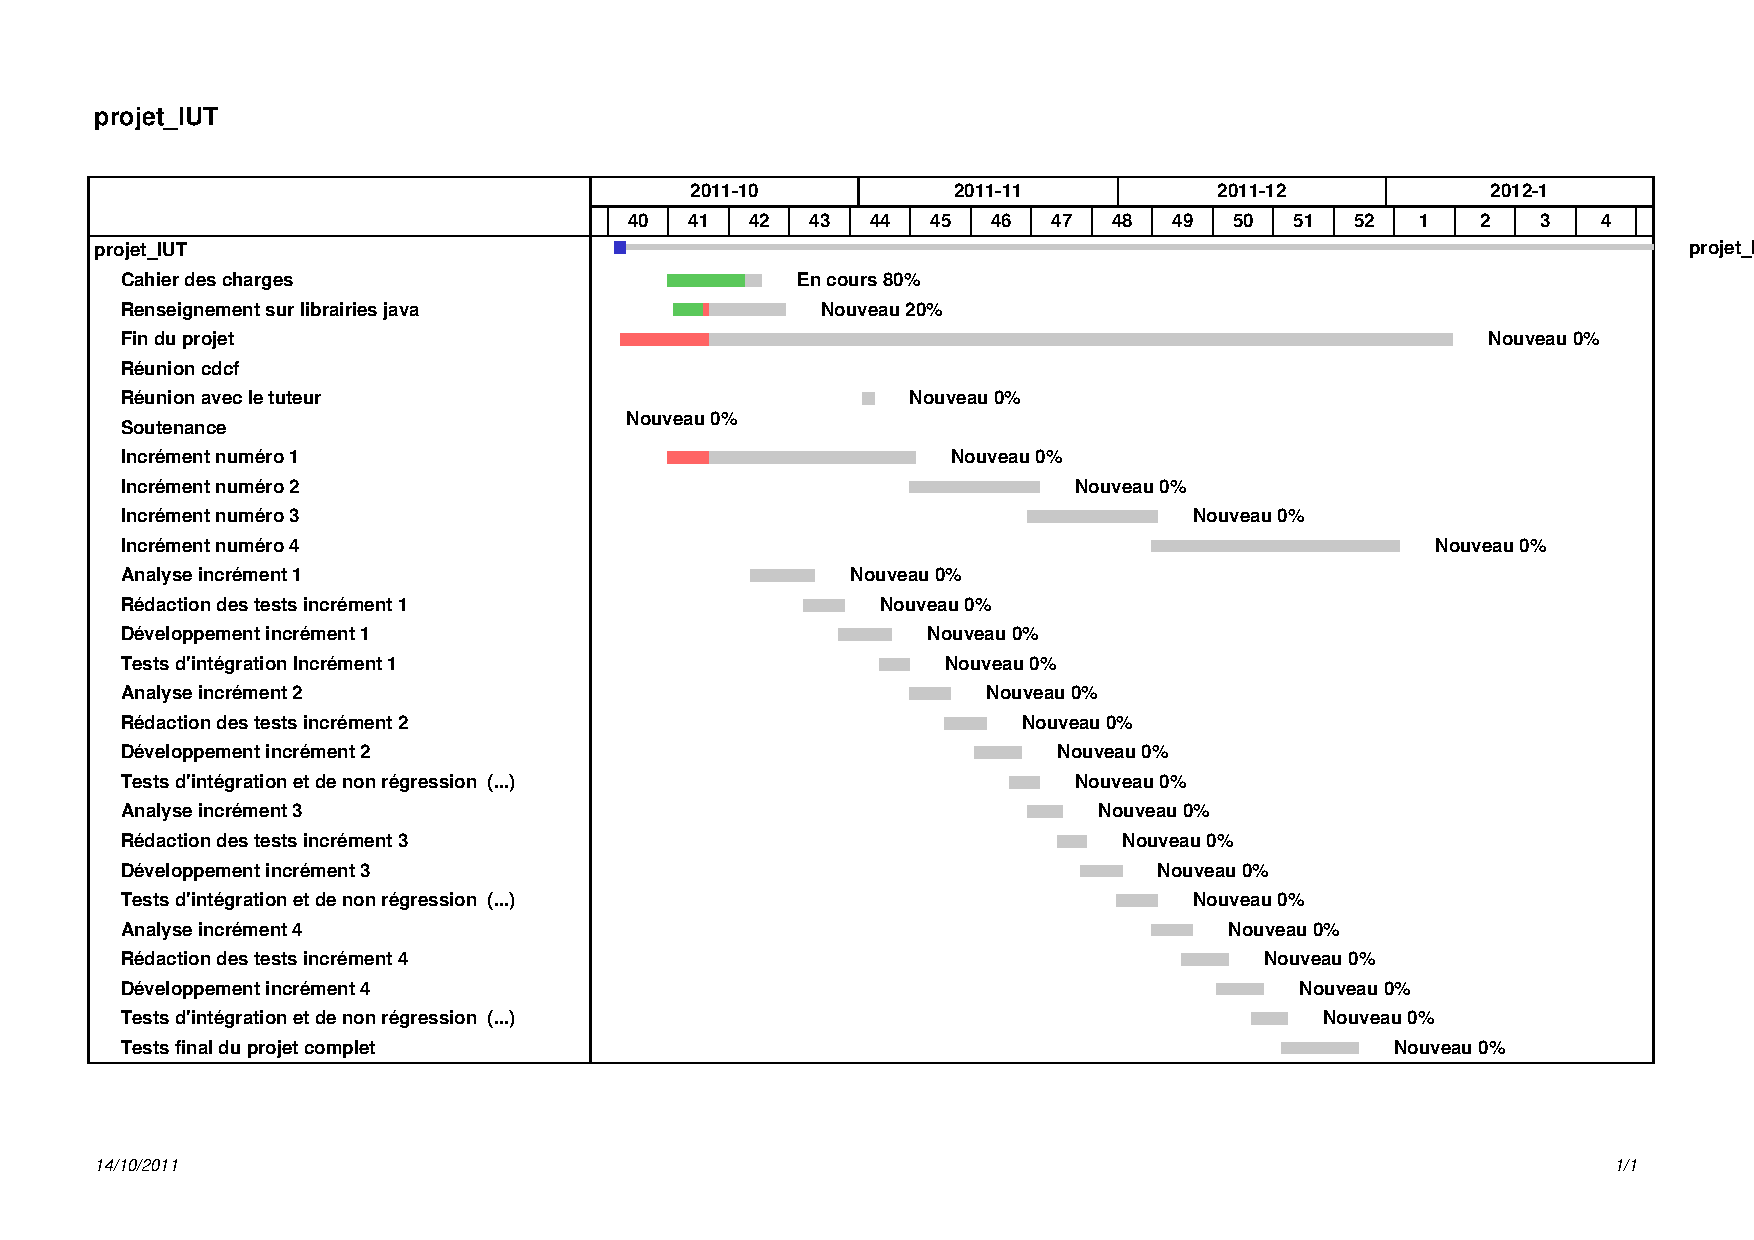
\includepdf[pagecommand={}, landscape]{projetiut-gantt.pdf}
	\subsection{Contraintes de ressources humaines}
	\begin{itemize}
		\item Le client doit valider chaque incréments et nous donner les directives pour l'incrément suivant afin de pouvoir continuer le projet. 
		\item Nous n'avons pas d'horaire aménagés pour le projet et nous n'habitons pas tous dans la même ville, ce qui peut poser des difficultés pour se voir, cependant nous aurons la possibilité de travailler à distance et le jeudi midi.
	\end{itemize}
	\subsection{Contraintes de ressources matérielles}
	\begin{itemize}
		\item Le projet devra être programmé en Java et utiliser l'EDI\footnote{Environnement de Développement Intégré} Netbeans. 
		\item Il devra être possible d'intégrer la bibliothèque en tant que composant dans un autre logiciel. 
		\item La documentation relative au projet ne devra pas être éditée sur support papier, nous utiliserons donc javaDoc pour produire une documentation 
	HTML\footnote{HyperText Markup Language}.  
	\end{itemize}
	
% Gantt => une réunion par semaine (projet) 
% Cahier des charges 
% Rendu du cahier des charges
% Réunion avec le client Lundi 17h
% Réunion avec le tuteur Mercredi 13h
% Tests d'intégration
% Rendez vous avec le client pour valider
% Soutenance + Fin projet 
% Après chaque incréments tests de non regression 
% Test avant le developpement
% Chaque incrément => Analayse
% incréments = deux semaines

\section*{Signatures}
\vspace{20px}
\begin{tabular}[center]{p{175px}p{175px}p{175px}}
  \textbf{Client :} & \textbf{Groupe :} & \textbf{Tuteur :} \\
  \\
  Le ~..................... & Le ~..................... & Le ~..................... \\
  A ~...................... & A ~...................... & A ~....................... \\
\end{tabular}
\end{document}
